\lhead{\emph{\leftmark}}  
\chapter{Background}
\label{chap:background}

This chapter presents the background knowledge required for readers to fully understand the subsequent chapters. The \textit{umplification} approach presented in this thesis is an incremental reverse engineering technique performing model transformations to transform base language program into Umple. In the following sections, we introduce the Umple language and we present the most important concepts about reverse engineering. 

\section{Umple Modeling Language}

Umple \cite{UmpleMAIN} is an open-source textual modeling and programming language that adds UML abstractions to base programming languages including Java, PHP, C++ and Ruby.

Umple has been designed to be general purpose and has UML class diagrams and UML state diagrams as its central abstractions. It has state-of-the art code generation and can be used incrementally, meaning that it is easy for developers to gradually switch over to modeling from pure programming. Umple was designed for modeling and developing large systems and for teaching modeling \cite{teachingUmple}. Umple is written in itself -- the original Java version was manually umplified many years ago. That experience was one of the motivations for the current work.
In addition to classes, interfaces and generalizations available in object oriented languages, Umple allows software developers to specify:
\begin{enumerate}
 \item 	\textit{Associations}: As in UML, these specify the links between objects that will exist at run time. Umple supports enforcement of multiplicity constraints and manages referential integrity – ensuring that bidirectional references are consistently maintained in both directions \cite{UmpleAssociations}.
 \item 	\textit{Attributes}: These abstract the concept of instance variables. They can have properties such as immutability, and can be subject to constraints, tracing, and hooks that take actions before or after they are changed \cite{UmpleAttributes}.
 \item \textit{	State Machines}: These also follow UML semantics, and can be considered to be a special type of attributes, subject to events that cause transitions from one value to another. States can have entry or exit actions, nested and parallel substates, and activities that operate in concurrent threads \cite{Badreddin2012_Thesis}.
 \item 	\textit{Traits}: A trait is a partial description of a class (containing elements such as methods, attributes and state machines) that can be reused in several different classes, with optional renaming of elements. They can be used to describe re-usable patterns.
 \item 	\textit{Patterns}: Umple currently supports the singleton and immutable patterns, as well as keys that allow generation of consistent code for hashing and equality testing.
 \item 	\textit{Aspect Oriented Code Injection}: This allows injection of code that can be run before or after methods, including Umple-defined actions on attributes, associations and the elements of state machines. Such code can be used as preconditions and post-conditions or for various other purposes. Code can be injected into the API methods (those methods generated by Umple) as well as into user-defined methods. 
 \item 	\textit{Tracing}:  A sublanguage of Umple called MOTL (Model-oriented tracing language) allows developers to specify tracing at the model level, for example to enable understanding of the behavior of a complex set of state machines operating in multiple threads and class instances \cite{UmpleTracing}.
 \item 	\textit{Constraints}: Invariants, preconditions and postconditions can be specified.
 \item 	\textit{Concurrency}: Umple provides several mechanisms to allow concurrency to be specified easily, including active objects, queuing in state machines, ports, and the aforementioned state activities.
\end{enumerate}

The Umple compiler supports code generation for Java, PHP, Ruby and C++, as well as export to XMI and other UML formats. The compiler generates various types of methods including mutator, accessor, and event methods from the various Umple features. A mutator (e.g. set(), add()) method is a method used to control changes to a variable and an accessor (e.g. get()) method is the one used to return values of the variable. An event method triggers state change. An extended summary of the API generated by Umple from attributes, associations, state machines and other features can be found at \cite{UmpleAPI}. Umple can also generate diagrams, metrics, and various other self-documentation artifacts. Umple models can be created or edited using the \textit{UmpleOnline} Web tool \cite{UmpleOnline}, the command line compiler or an Eclipse plugin. 

The umplification method discussed in this thesis currently focuses on associations,  attributes and state machines with some generation of code injections. The next sub-sections introduce these Umple constructs in greater detail.

\subsection{Umple Language Definition}
In this sub-section we present the grammar and metamodel defining the syntax and semantics of the Umple language. 

\subsubsection{Grammar}

Umple's language description is written in a slightly non-standard EBNF syntax. In standard EBNF grammars all tokens have to be strictly defined. Umple, however, supports blocks of code written in the different programming languages that don't need to be parsed. This means that an Umple developer/user can choose to embed a wide variety of blocks of native code within Umple code. The following are the main elements of the Umple grammar notation:

% You got a lot of the following few paragraphs about the grammar language completely wrong; I have corrected it, but it has alarmed me. Be extra careful about your facts, since I can't fact-check everything.
% MG. I will double check next time.

\paragraph{Non-Terminals} A \textit{rule-based} non-terminal uses double square brackets and represents a references to a another rule. In the example in Listing \ref{lst:grammarNT}, \textit{classContent} is a rule-based non terminal referring to the ClassContent rule. This allows reuse of such rules.  If the rule is declared with a minus sign following it, then the rule name is not added to the resulting tokenization string (abstract syntax tree) for simplicity; an example of this is found in \ref{lst:grammarExtra}. The definition of rule \textit{classContent} is shown in Listing \ref{lst:fullGrammar1}.

% Add the classContent rule to the Listing so people can see how it is used.
% MG Fixed. ClassContent is in listing fullGrammar1. I added the cross-reference to the text above.

\begin{lstlisting}[language={grammar}, label=lst:grammarNT,caption=Grammar for Umple classes]
 classDefinition : class [name] { [[classContent]]* }
\end{lstlisting}

\paragraph{Terminals} Terminals come in two types. Those shown in single square brackets match, by default, any alphanumeric string. In Listing \ref{lst:grammarNT}, \textit{name} is a terminal that matches an arbitrary alphanumeric string, and is expected to be followed by a curly bracket in this case. The second type of terminal is shown as actual text and guides the parsing. So for example in \ref{lst:grammarNT} 'class' is a terminal that must match exactly, as as are the open and close curly brackets. Note that the regular parentheses are metacharacters used for grouping, and the asterisk means means zero-or-more matches.

\paragraph{Native code blocks}
As we already discussed, blocks of native code are skipped. The rule in Listing \ref{lst:grammarExtra} defines the body of a method. The \textit{**code}  will match everything until the ending curly bracket is reached, while properly dealing with nested pairs of curly brackets found in the code. This allows the grammar to stay unchanged as new languages are added. 

In the following grammar examples, {\color{variableBlue}rules} are shown in blue, {\color{keywordRed}terminal} symbols are in red, {\color{stringGreen}identifiers} are in green and arbitrary input is in \textbf{black} and surrounded by [**]. 

\begin{lstlisting}[language={grammar}, label=lst:grammarExtra,caption=Grammar for Umple classes]
methodBody- : ( [[codeLangs]] { ( [[precondition]] | [[postcondition]] )* [**code] } )+
\end{lstlisting}

The grammar to parse classes (declarations), attributes, , and associations is presented in Listings \ref{lst:fullGrammar1}-\ref{lst:fullGrammar3} respectively.

A class definition starts with a name, followed by a curly bracket and any of the items in Lines 3-14 of Listing \ref{lst:fullGrammar1} such as attributes, state machines or inline associations. Note that for conciseness reasons, some rules have been omitted from Listing \ref{lst:fullGrammar1}. Additional details about the grammar metalanguage can be obtained in the online Umple user manual at \url{http://cruise.eecs.uottawa.ca/umple/UmpleGrammar.html}. The entire Umple grammar definition is located at \url{http://grammar.umple.org}.

% The listing has no line numbers - it ought to since you are referring to line numbers,
% MG. Fixed
% You should mention that additional details about the grammar metalanguage are located in the User Manual (give the exact URL) and that the entire Umple grammar is also located at http://grammar.umple.org
% MG. Added 

\begin{lstlisting}[language={grammar}, label=lst:fullGrammar1,caption=Umple Grammar for classes]
classDefinition : class [name] { [[classContent]]* }

classContent- : [[comment]] | [[abstract]] | [[keyDefinition]] | [[softwarePattern]] | [[depend]] | [[symmetricReflexiveAssociation]] | [[attribute]] | [[stateMachine]] | [[inlineAssociation]] |[[concreteMethodDeclaration]]| [[constantDeclaration]] [[invariant]] | [[exception]] |[[extraCode]]
\end{lstlisting}

\begin{lstlisting}[language={grammar}, label=lst:fullGrammar2,caption=Umple Grammar for attributes]
attribute : [[simpleAttribute]] | [[autouniqueAttribute]] | [[derivedAttribute]] | [[complexAttribute]]

simpleAttribute- : [=gpIdentifier:%]? [~name] ;
autouniqueAttribute- : [=autounique] [~name] ;
derivedAttribute- : [=modifier:immutable  |settable  |internal |defaulted |const |fixml]? [[typedName]] = ([[moreCode]] )+
complexAttribute- : [=unique]? [=lazy]? [=modifier:immutable |settable |internal |defaulted  |const |fixml]?[[typedName]] (= [**value])? ;
\end{lstlisting}

\begin{lstlisting}[language={grammar}, label=lst:fullGrammar3,caption=Umple Grammar for associations]
association : [=modifier:immutable]? [[associationEnd]] [=arrow:-- |-> |<- |>< |<@>- |-<@>] [[associationEnd]] ;
symmetricReflexiveAssociation : [[multiplicity]] self [roleName] ;
inlineAssociation : [=modifier:immutable]? [[inlineAssociationEnd]] [=arrow:-- |-> |<- |>< |<@>-  |-<@>] [[associationEnd]] ;
inlineAssociationEnd : [[multiplicity]] [~roleName]? [[isSorted]]?
singleAssociationEnd : [[multiplicity]] [type] [~roleName]? ;
associationEnd : [[multiplicity]] [=gpIdentifier:%]? [type] [~roleName]? [[isSorted]]?
multiplicity- : [!lowerBound:\d+|[**]] .. [!upperBound:\d+|[**]] | [!bound:\d+|[**]]
isSorted- : sorted { [priority] } : [=modifier:immutable]? [[inlineAssociationEnd]] [=arrow:-- 
  |-> 
  |<- 
  |>< 
  |<@>- 
  |-<@>] [[associationEnd]] ;
inlineAssociationEnd : [[multiplicity]] [~roleName]? [[isSorted]]?
multiplicity- : [!lowerBound:\d+|[**]] .. [!upperBound:\d+|[**]] | [!bound:\d+|[**]]
\end{lstlisting}

The complete set of grammar files, which are part of the source code of Umple \cite{umpleRepository}, can be found in the following directory:
% Make sure this reference umpleRepository is referring to github, not Google Code.
% MG. Verified.
\url{cruise.umple/src/*.*.grammar}

The intent of discussing the underlying grammar of Umple is to help provide context. To obtain a deeper appreciation for the capabilities of Umple one needs to understand the semantics, which we will outline in the following subsections.

\subsubsection{Metamodel}
Umple is represented internally using a metamodel that describes all the elements and their relationships. The Umple metamodel is developed in Umple itself; figure \ref{fig:umpleMetamodel} gives a sample from of the core of it. This class diagram was generated using Umple's internal diagram-drawing mechanism. As shown in the metamodel, an UmpleClass can be associated with many attributes, association variables and code injections. For a complete view of the Umple metamodel refer to \cite{UmpleMetamodel}.
% Tim, positioning of figure is fine when you download the pdf.

\begin{figure}[h]
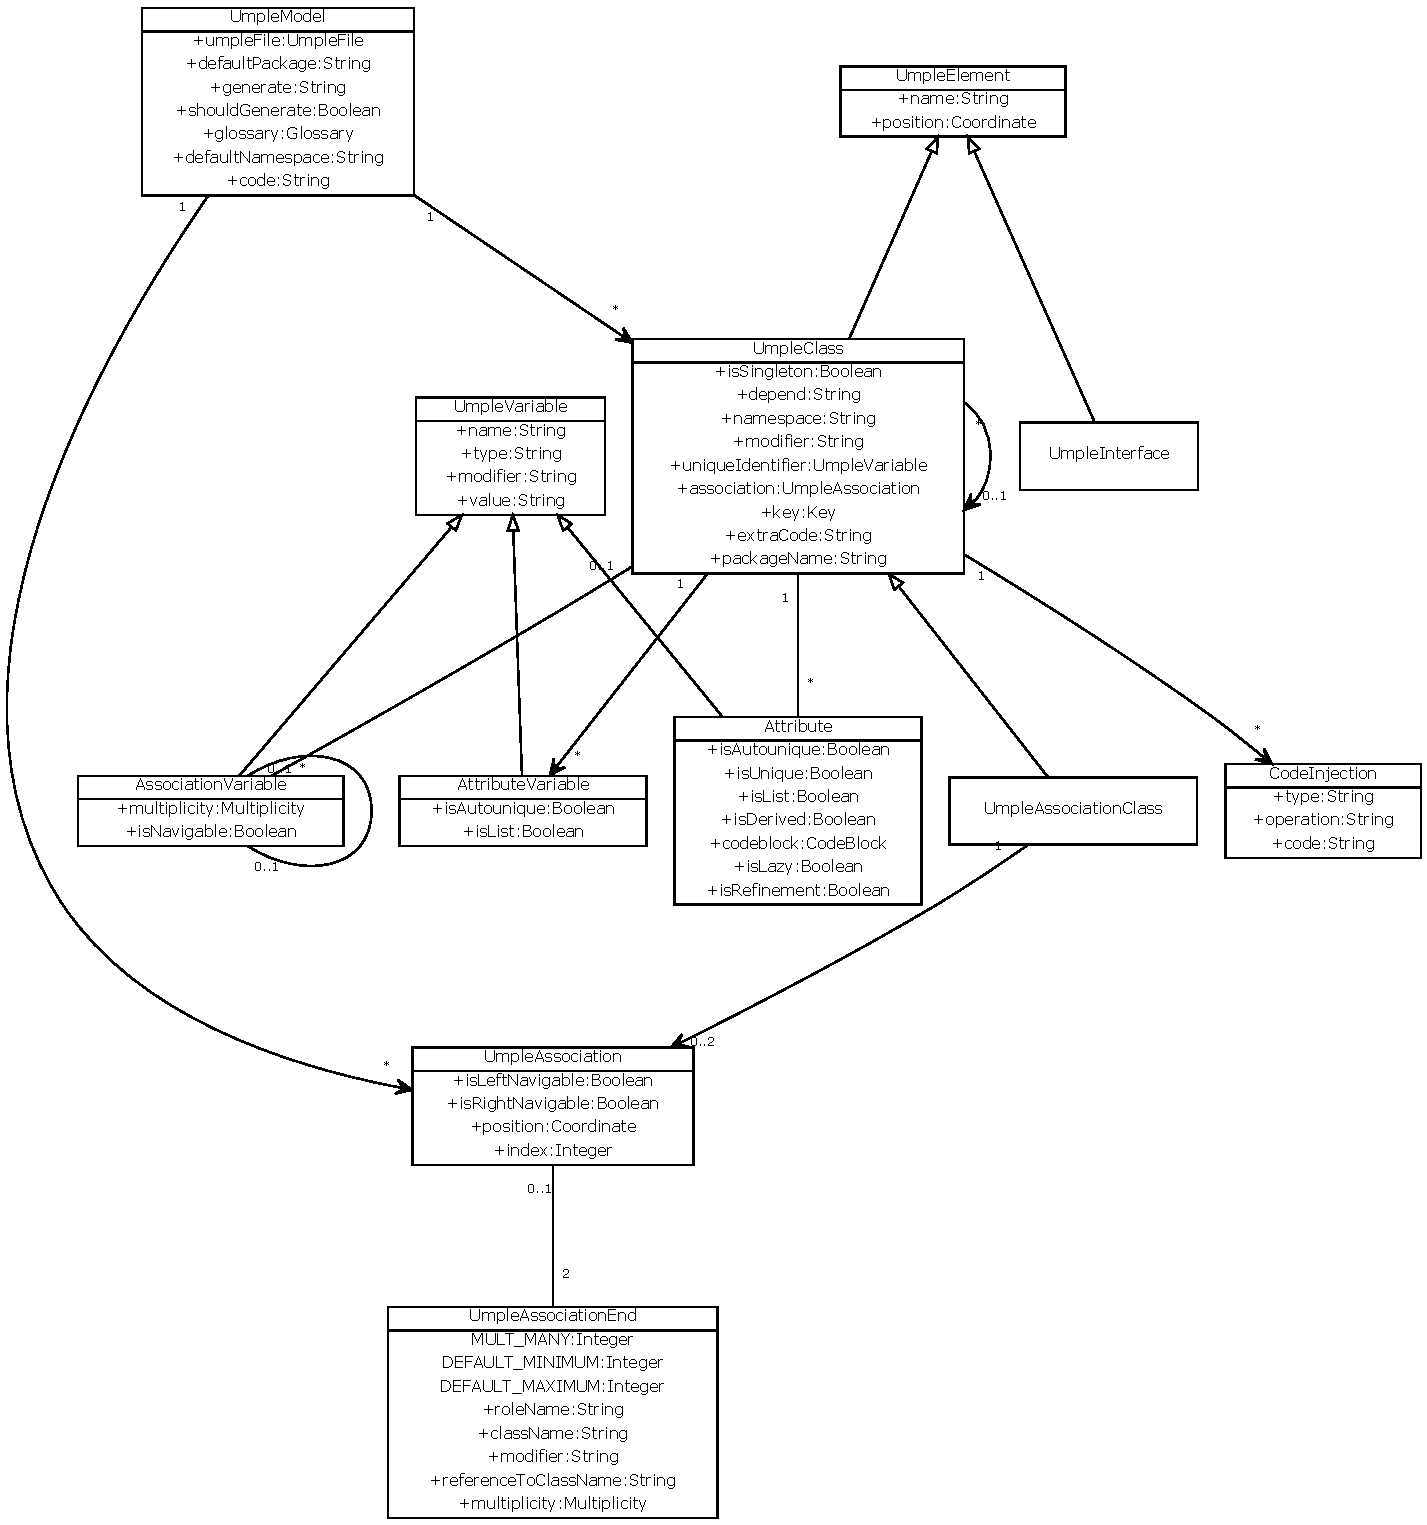
\includegraphics[width=1\textwidth]{Figures/metamodelUmple.pdf} 
\caption{Umple Metamodel (Partial)}
\label{fig:umpleMetamodel}
\end{figure}

\subsection{Umple Attributes}

An Umple attribute is a property of an object. For instance, 
a Person object might have a \textit{name} and an \textit{address}. 
An attribute can have various properties described in the following subsections.

\subsubsection{Basic Attributes}
A basic attribute in Umple represents simple data and is composed of one of the Umple data types and the name of the attribute. As shown in Tables \ref{table:apiAttrs1} and \ref{table:apiAttrs2}, the implications on code generation include a parameter in the constructor and a simple set and get methods to manage access to the attribute. The String datatype in Umple is the default type, when no type is specified. The example in in Listing \ref{lst:basicAttribute} shows multiple attributes having different (Umple) datatypes.

% Make the above explicitly reference the following listing, instead of saying 'below'. Same for the rest of the thesis.
% MG Fixed here and other parts

\begin{lstlisting}[style=umplePlain, label=lst:basicAttribute,caption=Basic Umple attribute]
class Demo 
{
  name; // String type
  Integer i;
  Float flt;
  String str;  
  Double dbl;
  Boolean bln;
  Date dte; 
  Time tme;
}
\end{lstlisting}

\subsubsection{Immutable Attributes}
The value of an immutable attribute can not change during the lifetime of an instance of the class. The resulting base language code (e.g. Java) for an immutable attribute would be the same as the basic attribute implementation except that there would be not setter method generated. A constructor argument is required so the value can be set at construction time but  cannot be changed afterwards since no setter is generated. The syntax for an immutable attribute is shown in Listing \ref{lst:immutableAttribute}. In this example, the \textit{studentId} must be initialized during construction and cannot changed after it. 

\begin{lstlisting}[style=umplePlain,label=lst:immutableAttribute, caption=Immutable Umple attribute]
class Student 
{
  immutable Integer studentId;
}
\end{lstlisting}

\subsubsection{Lazy and Immutable Attributes}
In cases where the attribute should be immutable, but the value is not available at the time of construction, the attribute can be declared as \textit{lazy immutable}. The use of the lazy syntax means that the attribute is not initialized in the constructor (i.e. it is not part of the constructor's signature). The generated code will contain a flag to track whether the object has been set yet, allowing only a single set to occur. In Listing \ref{lst:lazyimmutableAttribute},
attribute \textit{x} is declare as a lazy immutable attribute. The setter method of this attribute can be call once, since it will return false if we try to set it again (setter returns a boolean). Lazy immutable attributes are useful in architectures where the developer doesn't possess any control over the creation of the objects and therefore he can't specify constructor arguments.

\begin{lstlisting}[style=umplePlain,label=lst:lazyimmutableAttribute, caption=Lazy immutable Umple attribute]
class A 
{
  lazy immutable x;
}
\end{lstlisting}


\subsubsection{Defaulted attributes}
A defaulted attribute is set in the constructor to the default value, and can be reset to the default any time by calling a reset method (in this example \textit{resetName()}). It can be also set to any other value using its setter method. In Listing \ref{lst:defaultedAttribute}, the attribute 'name' is initializated to the default value 'UOttawa'. This default value can be queried by calling \textit{getDefaultName()}.

\begin{lstlisting}[style=umplePlain,label=lst:defaultedAttribute, caption=Defaulted Umple attribute]
class School 
{
  String name="UOttawa";
}
\end{lstlisting}

% You should talk about lazy and lazy immutable here, otherwise the reader will woner why you omitted them.
% MG Fixed. I added them before immutable

\subsubsection{Unique attributes}
The unique attribute guarantees its uniqueness within a particular class.
For instance, in the example in Listing \ref{lst:uniqueAttribute}, in the set method of attribute 'name', prior to setting its value , we will check for uniqueness. 

\begin{lstlisting}[style=umplePlain,label=lst:uniqueAttribute, caption=Unique Umple attribute]
class Student 
{
  unique String name;
}
\end{lstlisting}

\subsubsection{Autounique attributes}
The implementation of autounique attributes is very similar to the implementation of unique attributes presented in the previous sub-section. The main difference is that the autounique attribute is set in the constructor to the next available value. Autounique attributes must be of type Integer as shown in Listing \ref{lst:autouniqueAttribute}.

\begin{lstlisting}[style=umplePlain,,label=lst:autouniqueAttribute, caption=Autonique umple attributes]
class Student 
{
  autounique Integer studentId;
}
\end{lstlisting}

\subsubsection{Constant attributes}
A constant (class level) attribute is identified using the \textit{const} keyword as illustrated below. A constant is associated with the type itself, rather than an \textit{instance} of the type (i.e. it would be generated as a static variable in Java). Listing \ref{lst:constantAttribute} declares a constant of type Integer. 

\begin{lstlisting}[style=umplePlain,label=lst:constantAttribute, caption=Constants in Umple]
class Student 
{
  const Integer MAX_COURSES = 10;
}
\end{lstlisting}

\subsubsection{Array attributes}\emph{•}
Umple supports attributes that might contain multiple values. The square brackets notation '[]' is used as illustrated in Listing \ref{lst:arrayAttribute}.

\begin{lstlisting}[style=umplePlain,label=lst:arrayAttribute, caption=Array attributes]
class Student 
{
  String[] nickname;
}
\end{lstlisting}

In translating Umple attributes into object-oriented programming languages such as Java it is common to generate mutator and accessor methods. Tables \ref{table:apiAttrs1} and \ref{table:apiAttrs2} present the list of accessor and mutator methods generated from Umple attributes. In Tables \ref{table:apiAttrs1} and \ref{table:apiAttrs2}, T is the type of the attribute (String if omitted) and z is the attribute name.	

\begin{table}[h]
\centering
\caption{API generated methods from Umple attributes - Accessor  methods \cite{UmpleAPI}}
\label{table:apiAttrs1}
\begin{tabular}{lccc}
\toprule
\rowcolor[HTML]{BBDAFF}
\textbf{}               & \textbf{T getZ()}                                             & \textbf{boolean isZ()}     & \textbf{boolean equals(Object)} \\ \hline
      & returns the value                             & returns the value                                              & tests for reference equality    \\ \hline
\textbf{Basic}          & Yes                                                           & \begin{tabular}[c]{@{}l@{}}Yes;\\ if T is boolean\end{tabular} & No                              \\ \hline
\textbf{Initialized}    & Yes                                                           & \begin{tabular}[c]{@{}l@{}}Yes;\\ if T is boolean\end{tabular} & No                              \\ \hline
\textbf{Lazy}           & Yes                                                           & \begin{tabular}[c]{@{}l@{}}Yes;\\ if T is boolean\end{tabular} & No                              \\ \hline
\textbf{Defaulted}      & Yes                                                           & \begin{tabular}[c]{@{}l@{}}Yes;\\ if T is boolean\end{tabular} & No                              \\ \hline
\textbf{Immutable}      & Yes                                                           & \begin{tabular}[c]{@{}l@{}}Yes;\\ if T is boolean\end{tabular} & No                              \\ \hline
\textbf{Lazy immutable} & Yes                                                           & \begin{tabular}[c]{@{}l@{}}Yes;\\ if T is boolean\end{tabular} & No                              \\ \hline
\textbf{Autounique}     & \begin{tabular}[c]{@{}l@{}}Yes; \\ T always int.\end{tabular} & No                                                             & No                              \\ \hline
\textbf{Constant}       & No                                                            & No                                                             & No                              \\ \hline
\textbf{Internal}       & No                                                            & No                                                             & No                              \\ \hline
\textbf{Key}            & Yes                                                           & Yes                                                            & Yes                             \\ \hline
\end{tabular}
\end{table}

\begin{table}[h]
\centering
\caption{API generated methods from Umple attributes - Mutator methods \cite{UmpleAPI}}
\label{table:apiAttrs2}
\begin{tabular}{lcc}
\toprule
\rowcolor[HTML]{BBDAFF}
\textbf{}               & \textbf{boolean setZ(T)}                                  & \textbf{boolean resetZ()}                     \\ \hline
\textbf{Description}    & \multicolumn{1}{l}{mutates the attribute}                 & \multicolumn{1}{l}{restores original default} \\ \hline
\textbf{Basic}          & Yes                                                       & No                                            \\ \hline
\textbf{Initialized}    & Yes                                                       & No                                            \\ \hline
\textbf{Lazy}           & Yes                                                       & No                                            \\ \hline
\textbf{Defaulted}      & Yes                                                       & Yes;                                          \\ \hline
\textbf{Immutable}      & No                                                        & No                                            \\ \hline
\textbf{Lazy immutable} & \begin{tabular}[c]{@{}c@{}}Yes;\\ only once.\end{tabular} & No                                            \\ \hline
\textbf{Autounique}     & No                                                        & No                                            \\ \hline
\textbf{Constant}       & No                                                        & No                                            \\ \hline
\textbf{Internal}       & No                                                        & No                                            \\ \hline
\textbf{Key}            & Yes                                                       & No                                            \\ \hline
\end{tabular}
\end{table}

\subsection{Umple Associations}

In Umple, as in UML, an association defines a relationship from a class to another class. Furthermore, it specifies which links such as references or pointers may exist at run time between the different instances of the classes.
More specifically, an Umple association is composed of the following information:

\begin{itemize}
\item \textit{Association Ends}: These are the classes involved in the relationship.
\item \textit{Navigability:} The navigability determines whether or not the association can be accessed from the opposite end. The notation '--' is used when each class can access the linked objects of the other class and '-\textgreater{}' or '\textless{}-' to indicate that the navigation is possible in only one direction.
\item \textit{Multiplicity:} These are the restrictions on the numbers of objects allowed in the relationship.
\item \textit{Role names:} These are used to clarify the relationship and avoid name collisions if two classes are associated in multiple ways. Role names are optional except in reflexive associations or in other situations when name collisions might exist. The Umple compiler will give an error message if a role name is needed.
\end{itemize}

% In the following, refer to the listing by number
% MG Fixed.

The code segment in Listing \ref{lst:inlineAssoc} illustrates an association between instances of classes \emph{School} and \emph{Person}. In this example, an instance of class School can be associated to zero or more instances of class Student. The 'isA' notation is used to denote an inheritance relationship between the classes (Student is a subclass of Person). It should be noted that 'isA' is also used for other generalization relationships in Umple, such as implementation of Interfaces.

\begin{lstlisting}[style=umplePlain, caption=An example of an inline Umple Association, label=lst:inlineAssoc]
class School {
 0..1 -- * Student student; //inline association
}
class Student {
  isA Person;
}
class Person { }
\end{lstlisting}

Alternatively, in addition to defining an association embedded in one of the associated classes, it is also possible to specify an association independently as shown in Listing \ref{lst:externalAssoc}. 

\begin{lstlisting}[style=umplePlain, caption=An example of an independent Umple Association,label=lst:externalAssoc]
class School {
}
class Student {
  isA Person;
}
class Person { }

association {
 0..1 School -- * Student student;
}
\end{lstlisting}

In Tables \ref{table:apiAssocs1} and \ref{table:apiAssocs2}, we show the generated API methods for accessing and mutating the links in the association. X is the name of the current class, W is the name of the class at the other association end and r is a role name used when referring to W.

% I think in all these API tables, you should refer to the User Manual page, where they came from as a reference in the caption.
% MG. Done in all four tables.

\begin{table}[h]
\caption{API generated from Umple Associations - Accessor Methods \cite{UmpleAPI}}
\label{table:apiAssocs1}
\begin{tabularx}{\textwidth}{Y|Y}
\toprule
\rowcolor[HTML]{BBDAFF}
\textbf{Method Signature} & \textbf{Description}     \\ \hline
W getW() & Return the W;  \\ 
W getW(index) &	Picks a specific linked W;  \\ 
List \textless W\textgreater getWs() & Gets immutable list of links;  \\ 
boolean hasWs() & Returns true if cardinality is \textgreater  0; \\ 
int indexOfW(W)	 & Return index of W in the list;\\ 
int numberOfWs() & Return the cardinality;; \\ 
\end{tabularx}
\end{table}

\begin{table}[h]
\caption{API generated from Umple Associations - Mutator Methods \cite{UmpleAPI}}
\label{table:apiAssocs2}
\begin{tabularx}{\textwidth}{Y|Y}
\toprule
\rowcolor[HTML]{BBDAFF}
\textbf{Method Signature} & \textbf{Description}     \\ \hline
boolean setW(W)   & Adds a link to existing W   		\\ 
W addW(args)    & Constructs a new W and adds link      \\ 
boolean addW(W)  & Adds a link to existing W            \\ 
boolean setWs(W…)    & Adds a set of links              \\ 
 boolean removeW(W) &   Removes link to W if possible    \\
\end{tabularx}
\end{table}

%\subsection{Umple State Machines}
% if time allows.

\subsection{Code Injections}
Code injections are used to insert certain code statements \textbf{before} or \textbf{after} various Umple-defined actions on attributes, associations and (components of) state machines. Using \textbf{before} statements allows the developer to enforce preconditions and \textbf{after} statements to enforce postconditions. Code injections (after and before statements) can be added into the constructor, any user defined methods and into the API generated methods such as \textit{getX, setX, addX, removeX, getXs, numberOfXs, indexOfX}, where X is the name of the attribute or association.

\begin{lstlisting}[style=umpleOut,label={lst:codeInjection},caption=A code injection into the constructor]
class Operation {  
  const Boolean DEBUG=true;  
  query;  
  before constructor {  
    if (aQuery == null)  
    {  
      throw new RuntimeException("Please provide a valid query");  
    }  
  }  
  after constructor {  
    if (DEBUG) { System.out.println("Created " + query); }  
  }  
}  
\end{lstlisting}

The following gives details of the above:
\begin{itemize}
\item Line 2. Declares a constant (static final in Java). 
\item Line 3. Declares a simple (String) attribute.   	 
\item Line 4-9. Declares a code injection to be inserted at the beginning of the constructor.  
\item Line 10-12. Declares a code injection to be inserted at the end of the constructor.      
\end{itemize}

The code in Listing \ref{lst:codeInjection} generates the following (Java) constructor:

\begin{lstlisting}[style=java, caption=Generated constructor after code injection]
public Operation(String aQuery)
{
  if (aQuery == null)  
  {  
    throw new RuntimeException("Please provide a valid query");  
  }
  query = aQuery;
  if (DEBUG) { System.out.println("Created " + query); }
} 
\end{lstlisting}
% NEW
\subsection{Umple Architecture and Tools}

The Umple compiler, which was originally written in Java, was fully rewritten in Umple in 2008, and has been developed and maintained in Umple since then. 

The compiler has a layered and pipelined architecture as shown in Figure \ref{fig:umpleArchitecture}. 
The components of Umple includes: a parser, an analyzer as well as several code generators and model-to-model transformation engines. These are described below:

\begin{enumerate}
\item \textbf{Parser}: The parser receives an input model, written in Umple language, tokenizes it and passes it to the next component in the pipeline.

\item \textbf{Analyzer}: This component processes the tokens previously obtained and converts them into an internal representation consistent with Umple's metamodel. Errors and warnings are produced at this stage. Warnings mean that generation can occur, but there may be issues with the generated result. Errors mean that no code generation will be possible.

\item \textbf{Code-Generator(s)}: The internal representation is then translated into other artifacts; either additional models like Papyrus XMI, EMF, Yuml, Xuml; various diagrams, or source code such as Java, C++, PHP, Ruby or SQL. The compiler generates various types of methods including mutators (to control changes to a variable) and accessors (to return the value of a variable) from the various Umple features. Sophisticated code for managing state machines, tracing \cite{UmpleTracing}, generation templates, patterns, aspects and concurrency can also be generated from models.

\end{enumerate}
\begin{figure}[h]
\centering
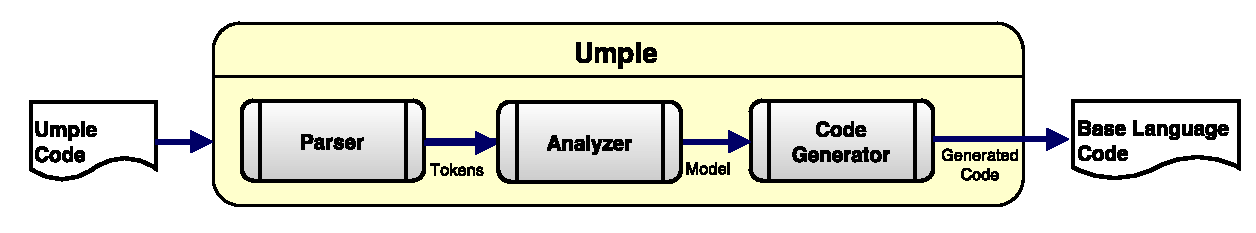
\includegraphics[width=0.99\textwidth]{Figures/umpleArchitecture.pdf} 
\caption{Umple Architecture}
\label{fig:umpleArchitecture}
\end{figure}

Each component is tested independently to ensure that the input is processed correctly and the output produced is valid. Testing the Umple parser is centered on tokenization of Umple code. Testing the metamodel classes ensures that the analyzer component produces valid metamodel instances. Testing of generated systems is also performed \cite{umpleTesting2014}.

% add a reference to our past paper on testing
% MG. Added above.

In addition to the Eclipse plugin and command-line based compiler, UmpleOnline \cite{UmpleOnline}, a web-based application shown in Figure \ref{fig:uonline}, allows to instantly experiment with Umple on the Web. 

\begin{figure}[h]
\centering
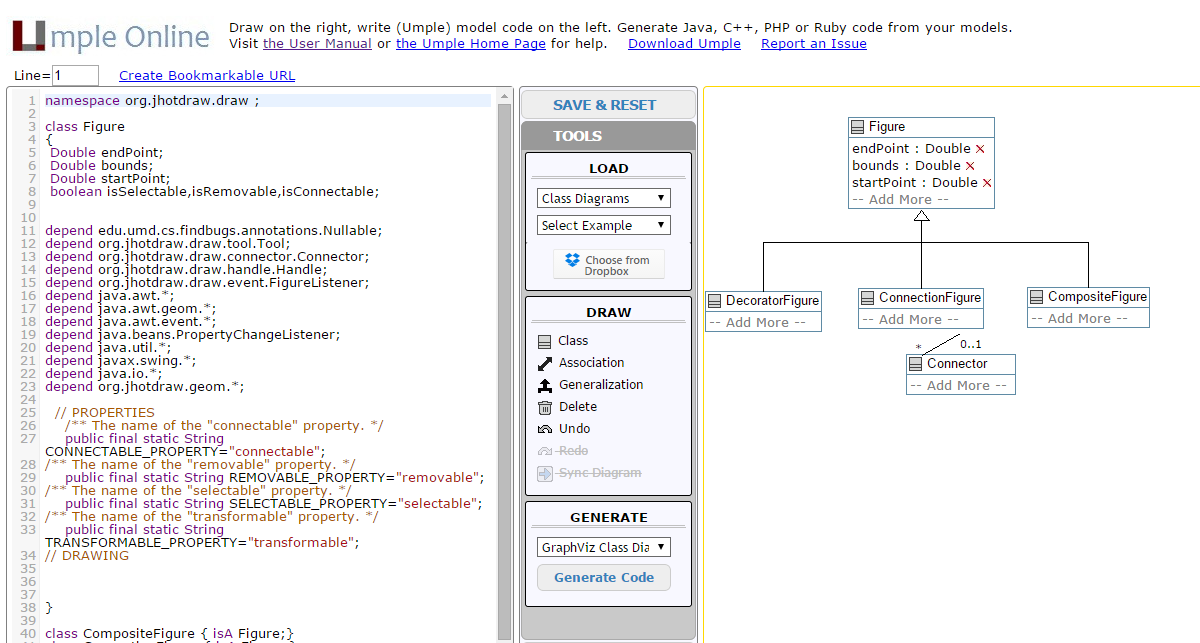
\includegraphics[width=0.75\textwidth]{Figures/uonline.png} 
\caption{Umple Online}
\label{fig:uonline}
\end{figure}
% END OF NEW

\section{Transformations}

In this section we will describe the different transformations that can occur during software design and implementation activities that are relevant to our research. In particular, we will present transformations that can occur during the design phase, during the implementation phase and when moving from one phase to another. Forward engineering, reverse engineering, model transformations and refactorings will be introduced in the following sections. The different transformations enumerated above are relevant to our work for the following reasons: 

\begin{itemize}
\item The umplification approach presented in this thesis is a \textit{reverse engineering} technique performing \textit{model transformations} to transform a base language model into an Umple model. 
\item The output of umplification is an Umple model. Umple models can be used to generate high quality code (\textit{Forward engineering}).
\item \textit{Refactorings} by means of umple code injections are required to adapt the different methods of an input class to conform to the Umple generated methods.
\item The umplification approach can be used in some measure to re-engineer an existing software system. A case study presenting a modernized software system is studied in the last section of Chapter \ref{chap:evaluation}.
\end{itemize}

To better conceptualize the different transformations, it is necessary to place them in the larger context of the software system lifecycle. As described in \cite{Chikofsky} and illustrated in Figure \ref{fig:re}, we assume a software life cycle with three main stages: Requirements, Design and Implementation. In the requirements phase, the problem being solved is specified, in the design phase the solution is specified using a well-defined model and in the implementation phase the code is produced from the previously obtained model. The work presented in this thesis as well as the related work studied focuses exclusively on the transformation that occur in the two last (abstract) stages of the life-cycle. Figure has been taken from \cite{Chikofsky} but has been simplified and modified for our purposes. As illustrated in Figure \ref{fig:re} the level of abstraction is higher in early stages and lower in later stages. Five different types of transformations can be distinguished:

\begin{figure}[h]
\centering
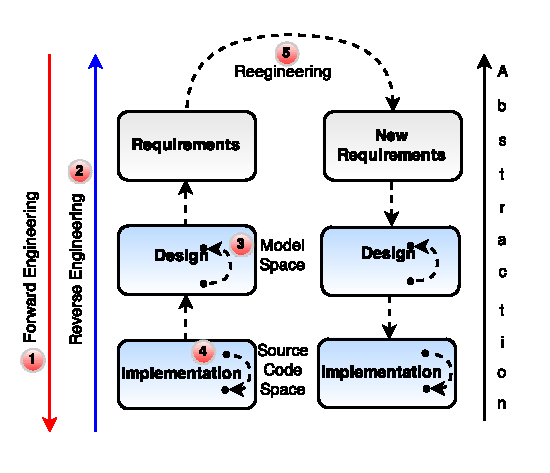
\includegraphics{Figures/transformationsRE}
\caption{Transformations across the different software life-cycle phases}
\label{fig:re}
\end{figure}

\begin{enumerate}
\item \textit{Forward engineering} produces source code corresponding to an object model. The modeling constructs in the model such as attributes, associations and high level constraints, are automatically mapped to source code constructs supported by the selected programming language. 
\item \textit{Reverse engineering} produces a model corresponding to source code. This transformation is often applied when the design of the system gas been lost and must be recovered. Reverse engineering can be seen as going backwards through the development cycle. Furthermore, reverse engineering does not involve changing aspects of the subject system. 
\item \textit{Model transformations} involve a conversion of an object model into another object model. 
\item \textit{Refactorings} involve transformations that operate on source code elements. Their goal is to improve aspects of the system without changing its functionality. They operate in the source code space.
\item \textit{Re-engineering} produces a new form of the subject system. 
\end{enumerate}

\subsection{Forward Engineering}

In Forward Engineering the target system is created by moving down from high-level abstractions to logic design and proceeds to the physical design of the system. As the of abstraction level decreases, information is collected about the system. The main goal of forward engineering is to maintain a strong correspondence between the object design model and the code and to reduce the development effort. 

\begin{quote} 
"Forward engineering is the traditional process of moving from high-level abstractions and logical, implementation-independent designs to the physical implementation of a system." \cite{Chikofsky}
\end{quote} 

Examples of forward engineering transformations include:

\begin{description}

\item [Mapping UML classes to Base language Classes]
Classes in the well-defined model (UML, Umple) are taken one by one and mapped into classes in the target programming language. 
\item [Mapping attributes to member variables]
Attributes in the model are mapped into member variables according to their characteristics. Implications on code generation in a object-oriented language such as Java, include a parameter in the constructor and mutator and accessor methods to manage access to the attribute.
\item [Mapping associations to Collections]
Associations, model concepts representing links between two or more objects are mapped into member variables and methods. Object-oriented programming languages do not support directly the concept of associations, they provide references to objects that can be stored. Associations are then realized in terms of references, taking into account the different parts of an association such as the role name, multiplicities and navigability. 
\item [Mapping Contracts to Exceptions]
Model constraints expressed in the model in \textit{OCL} or in natural language are mapped to code that checks the preconditions, postconditions and invariant in the target programming language.
\item [Mapping Object models to a persistent storage schema]
Object models are mapped to a storage schema. Attributes of the object models are mapped into columns and associations between the objects are mapped using a combination of primary and foreign keys. 
\end{description}

\subsection{Reverse Engineering}

Reverse engineering which involves extracting design artifacts and recovering models that are less implementation-dependent has been defined by Chikofsky and Cross \cite{Chikofsky} as:

\begin{quote} 
Reverse engineering is the process of analyzing a subject system to
\begin{itemize}
\item identify the system's components and their interrelationships and
\item create representation of the system in another form or at a higher level of abstraction
\end{itemize}
\end{quote}
Reverse-engineering are generally used to:
\begin{itemize}
\item Cope with complexity: understand large an complex systems.
\item Generate alternative views: automatically generate different ways to view systems
\item Recover lost information: extract what changes have been made and the reasons.
\item Detect side effects: help understand ramifications of changes.
\item Synthesize higher abstractions:  create alternative views that transcend to higher abstracts of software.
\item Facilitate reuse: detect candidate reusable artifacts and components.
\end{itemize}

Table \ref{table:approachesRE} summarizes the different reverse engineering approaches\cite{Chikofsky}: 

\begin{table}[h]
\caption{Summary of Reverse engineering approaches}
\label{table:approachesRE}
\begin{tabularx}{\textwidth}{X|X|X}
\toprule
\rowcolor[HTML]{BBDAFF}
\textbf{Approach} & \textbf{Description}  & \textbf{Related Techniques}  \\ \hline
Re-documentation & Is the creation or revision of a semantically equivalent representation within the same relative abstraction level. & Pretty Printers, Diagram generators, reference listing generators. \\ \hline

Design Recovery & Extracts design abstractions from a combination of code and existing documentation of the system. & Software metrics generators, static analyzers, dynamic tracers, visualization tools. \\ \hline

Restructuring & Is the transformation from one representation form to another at the same relative representation form to another at the same relative abstraction level, while preserving the system's external behavior & Source code analyzers, source code translators.   \\ \hline

Data re-engineering & Is the process of analyzing and is the process of analyzing and
reorganizing the data structures (and sometimes the data values) in a system to make it more understandable & Data model analyzers  \\ \hline

Refactorings & Is restructuring within an object-oriented context & Refactoring APIs \\ \hline  
 
\end{tabularx}
\end{table}

\subsection{Model Transformations}

Model transformation is a method that allows the automation of many activities like reverse engineering, refactoring, integration, analysis and simulation \cite{biehl2010literature}, which are used extensively in software development, maintenance and modernization. Model transformations are employed in tools such as code generators and parsers as well.

Kleppe et al. \cite{mccKleppe} provide a more formal definition of a model transformation:
\begin{quote}
A \textit{transformation} is the automatic generation of a target model from a source model, according to a transformation definition. 
\end{quote}
\begin{quote}
A transformation \textit{definition} is a set of transformation rules that together describe how a model in the source language can be transformed into a model in the target language.
\end{quote}
\begin{quote}
A transformation \textit{rule} is a description of how one or more constructs in the source language can be transformed into one or more constructs in the target language.
\end{quote}

Model transformations provide a mechanism for automatically creating or updating target models based on information contained in a source model, e.g. the generation of code from a UML model, the translation of a UML Class Diagram into an ER diagram or the translation of base language code into UML or any other textual or visual modeling language, such as Umple.
In order to perform a transformation between models, the models need to be expressed in a software language. This language can be specified by a \textit{grammar} or a \textit{metamodel}. As stated by Kleppe \cite{kleppe2007language}, grammars focus on the concrete syntax of the language while metamodels focus on the abstract syntax. Grammars are useful to describe the structure of the words in a language, metamodels are better in describing the language's concepts and its relations. Compared to metamodels, grammars have a strong mathematical basis (induction can be used to prove its correctness) and is tree based (e.g. parse trees are generated from grammar). Also, there are a great variety of tools advanced tools to produce, parse and validate grammars. On the other hand, metamodels are graph based in which relations between language elements are better perceived. Moreover, metamodels are more suitable when defining object-oriented languages but do not contain information on how the concepts in the metamodel are to be represented to the language user\cite{kleppe2007language}. Nevertheless, as studied by Alanen et al. \cite{alanen2003} it is possible to transform a grammar definition into a metamodel definition and vice-versa. In fact, the relation between a metamodel and a BNF grammar can in practise be defined using two mappings, one transforming a BNF grammar to a MOF metamodel,
and one transforming a MOF metamodel to a BNF grammar.

Previous work \cite{Czarnecki2006, biehl2010literature} model transformations allow us conclude that no model transformation tool or technique exists is \textit{absolutely} better than another one. Instead we can search for a model transformation approach that is suitable for a specific transformation problem. The following are the main properties of model transformation problems \cite{biehl2010literature}:

\begin{itemize}
\item Change of abstraction: Model transformations can change the level of abstraction between the source and the target model. That is, the transformation increase or decrease the level of details or leave it as unchanged.
\item Change of Metamodel: 
	\begin{itemize}
		\item In a \textit{endogenous} \cite{Visser2005} transformation both the source and target metamodels are 			the same.
		\item In a \textit{exogenous} \cite{Visser2005} transformation both the source and target metamodels are 			different.
	\end{itemize}
\item Supported technical spaces: Model transformations can operate between the metametamodel, metamodel and model levels \cite{OOPSLA2004Bezivin}. 
\item Supported number of models: A transformations can involved one (same source model resulting into a modified target model), two models (source and target models are different) and multiple models (several source models that produce a single target model).
\item Supported target type: The target model can be either text or another model. A Model-to-Text transformation create its target as a set of strings while a  Model-to-Model transformation create its target as an instance of the target metamodel.
\item Preservation of properties: Transformations can be performed in such a way that the source and target model have a common property that is not transformed by the transformation \cite{biehl2010literature}. The intent of that common property can be to preserve the semantics, syntax or behavior of the source and target models. 
\end{itemize}

Based on the target type supported, we categorized the model transformations approaches into two major categories\cite{Czarnecki2006}: Model-to-Model and Model-to-Text approaches. 

\subsubsection{Model-To-Text Approaches}
\begin{description}
\item[Visitor-Based Approaches]
An approach based on the notion of traversing the internal representation of the model. The output is written to a text stream. The approach is based on the Visitor software pattern \cite{gamma1994design}. 
\item[Template-Based Approaches]
Template-based approaches are used in the implementation of code generators. The basic idea is to refine and transforms models into code. The templates contain fragments of the target text and pieces of code that are replaced with information derived from the source model (called meta-programs). This approach can be combine with the visitor-based approach for model traversing. 
\end{description}

\subsubsection{Model-To-Model Approaches}
\begin{description}
\item[Direct-Manipulation Approaches] The approach typically consist of an internal representation of the model (e.g. AST) and some API's to manipulate and query it. Modisco \cite{ModiscoMain} technology falls under this category.
\item[Structure-Driven Approaches]
The basic idea behind this approach is to copy model elements from the source to the target, which can  then be adapted to achieve the transformations goals. The approach is structure-driven because this approach first creates the hierarchical structure of the target model. \textit{OptimaJ} frameworks is one of the representative technologies falling under this category.
\item[Operational Approaches]
Operational approaches extend the metamodeling formalism with facilities for expressing mapping rules. 
Imperative approaches focus on how the transformation itself needs to be performed. Operational transformation languages provides support to describe how the transformation language is supposed to be executed. The constructs and concepts of an imperative language are similar to those of general purpose programming languages such as Java. The model trans-formation in this case is described as an ordered sequence of actions. \textit{Kermeta} and \textit{QVT} presented later in this chapter are examples of technologies in this category.
\item[Declarative Approaches]
Declarative approaches do not offer explicit control flow. They don't describe how the trans-formation should be executed but instead what should be mapped by the transformation. In other words, they describe the relationship between the source and the target metamodels. The transformation descriptions (or mapping rules) for these languages are, in general, short and concise. 
\item[Hybrid Approaches]
Hybrid transformation languages are a mix of declarative and operational approaches and offer the possibility of declaring how and what elements of the metamodels are going to be mapped \cite{HybridModelTransform}.
\item[Graph-Transformation-Based Approaches]
Graph-based approaches can be considered as a special subcategory of declarative languages. Models are interpreted as graphs, and the transformation manipulates these graphs \cite{GraphTransformations2006}. For instance, the Triple Graph Grammar (TCG) \cite{GraphTransformations2006} is a way of describing graph transformations. Their rules are specified using three graphs, the left-hand side graph corresponding to the source graph, the right-hand side graph corresponding to the target graph and a correspondence graph describing the mapping between elements of the left-hand side and elements of the right-hand side.
\item[XML Approaches]
In this approach models are serialized as XML and then traversed and transform using XSLT. However, the use of XMI and XSLT has scalability limitations \cite{peltier2001mtrans}. 
\end{description}

\subsubsection{Model Transformations Languages and Tools}

We now introduce some of the most popular existing model transformation technologies.

\begin{description}
\item[ATL]
The ATLAS Transformation Language \cite{atl} is a hybrid model-to-model trans-formation language supporting both declarative and imperative constructs. ATL is integrated in the Eclipse development environment and can handle models based on EMF (Ecore). The ATL code (.atl files) is compiled and then executed by its own transformation engine. Examples of Java-to-Umple ATL transformations will be presented in Chapter \ref{chap:tool}.

\item[QVT]
The QUERY/VIEW/Transformation \cite{QVTMain} is a standardized language for model transformation established by the Object Management Group (OMG). QVT defines three syntaxes for model-to-model transformations: a textual concrete syntax a XMI based metamodel and visual syntax for matching element between metamodels.
Listing \ref{lst:QVTExample} shows a partial transformation from an UML class model to an Umple model.

\begin{lstlisting}[style=java,label=lst:QVTExample, caption=A basic QVT transformation]
transformation uml2Umple(
 in uml : SimpleUML,
 out umple : SimpleUmple
);

main() {
  uml.objectsOfType(Class)->map UMLClassToUmpleClass();
}

mapping Class::classToUmpleClass () : UmpleClass
{
  name := self.name;
  attributes : self.attributes->map attributeToUAttribute();
}

mapping Attributes::attributeToUAttribute () : Attribute {
 ... omitted
}
\end{lstlisting}

The following gives details of the above:

\begin{itemize}
\item Lines 1-4. The transformation declaration specifies the parameter models. The transformation is unidirectional from UML to Umple.
\item Line 6. The entry point for the execution is the function \textit{main()}, which invokes the \textit{UMLClassToUmpleClass} mapping on all UML classes. 
\item Lines 10 and 16. The mappings are defined using the OCL notation. The attributes of each UML class are traversed and converted to Umple attributes (code is omitted). The body of the mapping populates the properties of the return object, while self refers to the object on which the mapping is invoked.
\end{itemize}
\item[JET]
Java Emitter Templates (JET) is a generic template engine that can be used to generate SQL, XML, Java source code and other output from templates. The templates uses a JSP-like syntax.
For instance, the code in Listing \ref{lst:JETExample} will print the words "Hello, Thesis Reader!" to the standard console output. The JET Builder translates the template to a class named BasicTemplate. The template file receives a string argument.

\begin{lstlisting}[style=java,label=lst:JETExample, caption=A basic JET Template]
<%@ jet package="hello" class="BasicTemplate" %>
 Hello, <%=argument%>!
\end{lstlisting}

To pass arguments to the template method we use the generate \textit{method} as shown in Listing \ref{lst:JETExample2}. Note that is possible to pass a reference (a model element) type as argument. 

\begin{lstlisting}[style=java,label=lst:JETExample2, caption=Instantiating the BasicTemplate class]
 BasicTemplate sayHello = new BasicTemplate();
 String result = sayHello.generate("Thesis Reader");
 System.out.println(result);
\end{lstlisting}

\item[Kermeta]
Kermeta \cite{kermetaMain} is an imperative programming language used to perform model transformations and for other more general purposes. It offers EMF meta-modeling, checks and behavior support. Incremental model transformations are supported. The Kermeta language uses metamodel-based actions to manipulate elements from different metamodels (in XMI format) and transform them. 

\item[ETL]
ETL \cite{ETLMain}  is a hybrid model-to-model transformation language. It can handle several source and several target models. It offers support for query/navigate/modify both source and target models. It works at the metamodel level and support EMF models. 

\item[TXL]
TXL \cite{Cordy2006}  is a programming language designed for a variety of analysis and source transformation tasks. TXL is a hybrid rule-based language and it is best at tasks involving source-to-source transformations.  Examples of Java-to-Umple TXL transformations will be presented in Chapter \ref{chap:tool}.
\end{description}

Table \ref{table:toolSummary} summarizes the most representative tools for each model transformation approach discussed.

\begin{table}[h]
\caption{Summary of Model transformation technologies}
\label{table:toolSummary}
\begin{tabularx}{\textwidth}{X|X}
\toprule
\rowcolor[HTML]{BBDAFF}
\textbf{Tranformation Approach} & \textbf{Technologies}     \\  \\ \hline
M2T- Visitor-Based Approaches & Jamada, CodeWirters  \\  \\ \hline
M2T- Template-Based Approaches  & JET, Velocity, XDoclet, Codagen  \\ \\ \hline
\hline
Direct-Manipulation Approaches & JML   \\ \hline
Structure-Driven Approaches & QVT, OptimalJ   \\ \hline
Operational Approaches & XMF-Mosaic, QVT-Relational, Kermeta  \\ \hline
Declarative Approaches & ATL, ETL    \\ \hline
Hybrid Approaches & CSCWMDA   \\ \hline
Graph-Based Approaches & AGG, AToM3,VIATRA, GReAT, UMLX, BOTL, MOLA, and Fujaba  \\ \hline
XML Approaches & XSLT   \\ \hline
\end{tabularx}
\end{table}

\subsection{Refactorings}

A \textit{refactoring} is a transformation of the \textit{source code} aiming at improving its readability and/or design of the code without changing the behavior of the system \cite{Fowler2000}. To ensure that the refactoring does not change the behavior of the system, the refactoring is done in small incremental steps that are interleaved with tests. 
For example, a sequence of three refactorings are performed to the source code in Listing \ref{lst:refactoring}.
The resulting source code after the transformations is presented in Listing  \ref{lst:refactoring2}. The refactorings are performed one by one and ensuring that the refactoring do not change the intended behavior of the system.For a complete catalog of  refactorings refer at \cite{Fowler2000}. 

\begin{enumerate}
\item Pull Up Field: Common field in subclasses is moved to the superclass. In our example, field \textit{name} is moved to superclass. 
\item Pull up Constructor: Common code in constructor bodies of subclasses is moved to the superclass constructor. 
\item Pull up Method: Methods with identical results on subclasses are moved to superclass. In our example, the methods accessing the \textit{name} field are moved from the subclasses to the superclass. 
\end{enumerate}


\noindent\begin{minipage}{.45\textwidth}
\begin{lstlisting}[style=java,caption=Before refactorings,label=lst:refactoring]{Name}
public class Student {
  private String name;
  public Student(String name) {
   this.name = name;
  }
  public String getName() {
	return name;
  }
}
///----- Class Mentor ------
public class Mentor {
  private String name;
  public Mentor(String name) {
   this.name = name;
  }
  public String getName() {
	return name;
  }
}
\end{lstlisting}
\end{minipage}\hfill
\begin{minipage}{.45\textwidth}
\begin{lstlisting}[style=java,caption=After refactorings,label=lst:refactoring2]{Name2}
///----- SuperClass ------
public class Person {
  private String name;
  public Person(String name) {
   this.name = name;
  }
  public String getName() {
	return name;
  }
}
///----- Class Student ------
public class Student extends Person {
  private String name;
  public Student(String name) {
   super(name);
  }
}
///----- Class Mentor ------
public class Mentor extends Person {
  private String name;
  public Mentor(String name) {
   super(name);
  }
}
\end{lstlisting}
\end{minipage}

\subsection{Re-engineering}

Re-engineering is the examination and alteration of a subject system to reconstitute it in a new form \cite{Chikofsky}. 
Re-engineering transformations are usually concerned with reimplementing a system (or parts of it) to make it more maintainable. Re-engineering involves redocumenting the system, organizing and restructuring the system or translating the system to a more modern programming language, know as modernization. Modernization is performed to extract the main components of the system, written in old (legacy) code, and to reproduce the original system using a more recent programming language or using modern frameworks and libraries.

The main activities in a typical re-engineering process are:

\begin{description}
\item[Source code Translation]
The most simple form of re-engineering is source code translation and involves the automatic translation of source code written in one programming language to source code in another (i.e., C to C++). The translation should not modify the structure and organization of the system. Source code translation can be done to the same but more modern version of the language (i.e.,Java 1.4 to Java 1.8). A source code translation is very desirable when the language compiler or support is discontinued or when the organization policies impose a change on the language (i.e., Microsoft technologies to Open source technologies). Furthermore, systems written in modern languages are often easier to understand, test and maintain than legacy systems \cite{Pressman2001}.

\item[Reverse Engineering]
Reverse Engineering can be used as part of the Reengineering process to recover the original program design. The design can then help developers understand the program internals before attempting to improve it. As originally explained by Chikofsky  \cite{Chikofsky}, reverse engineering and reengineering differ in their purpose. The main goal of reverse engineering is to derive the specification or design of a system from its source code, while the purpose of reengineering is to produce a new but more maintainable system. 

\item[Program Improvements]
This part of the reengineering process involves improving the structure of the program to optimize memory use or to simplify the logic structure of the system. 
\end{description}

In the following chapter, we will describe the core concept of this thesis, the umplification technique, a \textit{reverse engineering} technique that employs \textit{model-to-model transformations} to  incrementally transform base language code into Umple code.